\documentclass[11pt]{amsart}

\usepackage{mathptmx}
\usepackage{a4wide}
\usepackage{graphicx}

\begin{document}

\section{Classification results}

\begin{center}
  \begin{tabular}[c]{llll}
    \hline
    \texttt{1716.bases}
    & Team Bearland
    & yes
    & 0.33 s
    \\
    & Tresplans
    & yes
    & 0.210 s
    \\
    & other-awesome-team-name
    & yes/no
    & [seconds]
    \\\hline
      \texttt{252.bases}
    & Team Bearland
    & yes
    & 0.007 s
    \\
    & Tresplans
    & yes
    & 0.004 s
    \\\hline
      \texttt{3432.bases}
    & Team Bearland
    & yes
    & 1.276 s
    \\
    & Tresplans
    & yes
    & 0.810 s
    \\\hline
      \texttt{4092.bases}
    & Team Bearland
    & no
    & 0.019 s
    \\
    & Tresplans
    & no
    & 0.001 s
    \\\hline
      \texttt{417.bases}
    & Team Bearland
    & no
    & 0.002 s
    \\
    & Tresplans
    & no
    & 0.001 s
    \\\hline
      \texttt{462.bases}
    & Team Bearland
    & yes
    & 0.021 s
    \\
    & Tresplans
    & yes
    & 0.130 s
    \\\hline
      \texttt{4639.bases}
    & Team Bearland
    & no
    & 0.397 s
    \\
    & Tresplans
    & no
    & 0.001 s
    \\\hline
    \texttt{6435.bases}
    & Team Bearland
    & yes
    & 4.506 s
    \\
    & Tresplans
    & yes
    & 2.861 s
    \\\hline
    \texttt{924.bases}
    & Team Bearland
    & yes
    & 0.088 s
    \\
    & Tresplans
    & yes
    & 0.070 s
    \\\hline
  \end{tabular}
\end{center}

\section{Execution times}

\subsection{Team Bearland}

We implemented a mask-based algorithm.
Each mask $m$ represents a set.
The $i$-th bit of the mask is set to 1 iff $i$ belongs to the set.
We can easily, and in a fast manner, access each position shifting bits, and unions, intersections and complements are solved using bitwise OR, AND, NOT, and XOR operators.
The code implemented in \textsc{Python3}, albeit leveraging the same principle, implements the masking operations differently.
 
In both cases, the complexity is the same. We take advantage of the fact that all values in all inputs are integers between $0$ and $r - 1 = 19$. In every case, we build the masks in $\mathcal{O}(\sum_{B \in \mathcal{B}} |B|) = \mathcal{O}(r|\mathcal{B}|)$ time. Then, for each pair $(B_1, B_2) \in \mathcal{B} \times \mathcal{B}$, we check that the exchange conditions by taking all $\mathcal{O}(r)$ values of $x \in B_1$, and checking if the condition holds for each of the $\mathcal{O}(r)$ possible values of $y \in B_2$, and we also check that $x \in B_1 \setminus B_2$ and $y \in B_2 \setminus B_1$ in $\mathcal{O}(r^2)$ time. Finally, we check that the mask for $B_1 \setminus \{x\} \cup \{y\}$ belongs to the set of masks in $\mathcal{O}(\log(|\mathcal{B}|))$ time. Therefore, the total complexity is $\mathcal{O}(r |\mathcal{B}|) + \mathcal{O}(r^2 |\mathcal{B}|^2| \log(|\mathcal{B}|)) =  \mathcal{O}(r^2 |\mathcal{B}|^2| \log(|\mathcal{B}|))$.

Figure~\ref{fig:team-bearland-times} summarizes the execution times for both programming languages.
Note that we re-ordered the results to plot them in a, more or less, increasing fashion. 
\begin{figure}[h!]
    \centering
    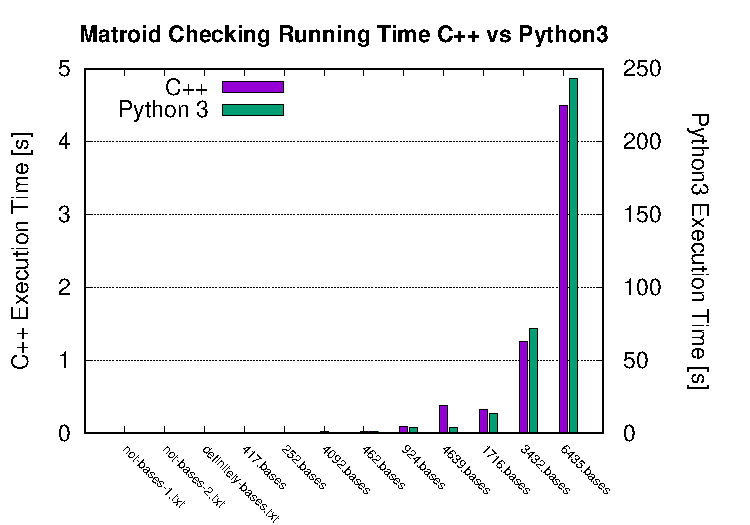
\includegraphics[width=.7\textwidth]{./team-berland/exec_time.pdf}
    \caption{Execution time of the two different implementations in increasing order.\label{fig:team-bearland-times}}
\end{figure}
The results were to be expected, the compiled, performance-oriented, \textsc{C++} implementation outruns the \textsc{Python3} one by two orders of magnitude.
However, we do observe that the behaviour, the pattern described by execution times as we increase the load (\textit{i.e.} the complexity) is the same for both algorithms.
This is a great example not to underestimate the constants affecting our expected running time, usually disregarded by complexity theory and big $\mathcal{O}$ notation.
%Under our point of view, each programming language has it's 

\subsection{Tresplans}

We implemented an algorithm based on hash tables (dictionaries in python).
In order to convert each integer list into a distinct key,
we stored each digit as a shifted bit into a bit array,
the whole list is then the sum of all bits (with an OR operation).
This method gives us distinct keys for each list of integers.
With this method,
we have been able to process all files.

Then, we can check if a list of bases exist in the hash table in a constant time.
The operation
\(x \in B_1 \setminus B_2\)
is implemented as
\(B_1 \land \neg B_2\)
on the bit array and selecting digits on the resulting bit array
(similar for \(y\)).
The operation
\(B_1 \setminus \{x\} \cup \{y\}\)
is also implemented as
\(B_1 \land \neg \{x\} \lor \{y\}\).

The complexity of our code is the same in both implementations.
It can be computed as follows, where $N$ is the number of bases:

\begin{itemize}
 \item Process file: $O(N)$.
 \item Compare bases: $O(N^2)$.
 \item Compare each pair of subsets of the base:
       constant time, with a large constant.
\end{itemize}

Thus, overall complexity is $O(N^2)$.
It is also output-sensitive,
as it stops if it finds a pair of bases do not satisfy the exchange axiom.

In figure~\ref{fig:Tresplans} we have the running time of both implementations.

\begin{figure}[h!]
    \centering
    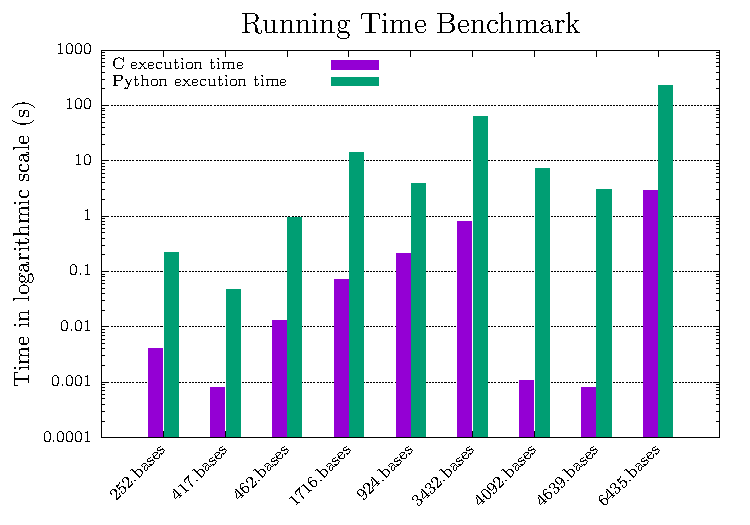
\includegraphics[width=.75\textwidth]{./Tresplans/Tresplans_exec_time.pdf}
    \caption{Execution times of the different implementations.
    \label{fig:Tresplans}}
\end{figure}

Time is displayed in logarithm scale to be able to compare it better,
as the values have a large span either between the same implementations,
and within the same implementation with different files.
Note that as the algorithm is output-sensitive,
a larger file not always leads to larger execution times,
as if there is a pair of bases that do not satisfy the exchange axiom,
then the routine exits.

It is clear that the \textsc{C} implementation is much faster in all cases.
The \textsc{Python} implementation takes a long time to build the dictionary.
It can be observed as the running time is much similar to the
\textsc{C} implementation when the file is large.
Also, most of the difference is because \textsc{Python} checks the type
of the variables in running time,
while in the case of the \textsc{C} code,
it does not happen and mostly works with memory addresses.

In both cases,
due to the complexity of the algorithm
and the fact that in each iteration we need to do a lot of operations and checks,
the execution times grow orders of magnitudes when comparing different files.

\subsection{other-awesome-team-name}

another plot here

\end{document}
